The units and uncertainties of the properties in this section are set here. The energy unit is eV with uncertainty $\pm$ 0.003 eV, pressure is in units kbar with uncertainty $\pm$ 1 kbar and force in units eV/Å with uncertainty $\pm$ 0.01 eV/Å.


\subsection{Primitive unit cell}

With the initial decided convergence criteria and the resulting energy cut-off (600 eV) and k-point density (5 Å$^{-1}$), we relaxed the primitive unit cell. Table \ref{tab:ionstep_primitive} shows both the maximum force and the pressure decreasing (ISIF = 3). The relaxation criteria for the force was set to -0.01 eV/Å (EDIFFG = -0.01).

\begin{table}[H]\caption{This table lists the start and stop of the relaxation of the primitive unit cell. Both the maximum force, F$_{max}$, and the pressure, P, is decreasing in the relaxation.}\label{tab:ionstep_primitive}
\begin{tabular}{ccccc}
F$_{max}$ &\#$_{atom}$&	P&	Drift&	E$_{tot}$\\ \hline
1.716&	9&	139.52&	0.000&	-119.461\\
$\vdots$&$\vdots$&$\vdots$&$\vdots$&$\vdots$\\
0.006&	9&	0.42&	0.000&	-120.224\\
\end{tabular}
\end{table}

The total energy per atom with a primitive unit cell was $\frac{E_{tot}}{\# \text{ of atoms}} = \frac{-120.249 \text{ eV}}{20} \simeq -6.013 \text{ eV}$ after the relaxation.

\subsubsection{Density of States}

To examine the different oxygen sites, the local density of states (DOS) was plotted for the inequivalent sites. The local DOS plots for the O(I), O(II) and O(III) are in Figure \ref{fig:ldos_Ga_I}, Figure \ref{fig:ldos_O_II} and Figure \ref{fig:ldos_O_III} respectively.

\begin{figure}[H]
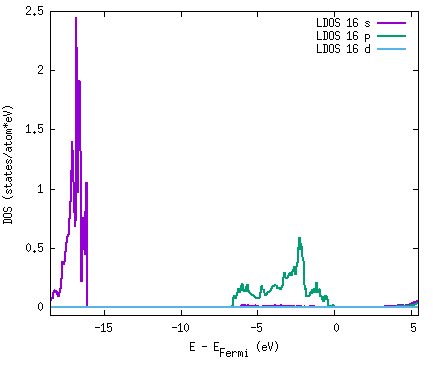
\includegraphics[width=\linewidth]{../fig/dosplot/ldos_O_I_primitive}\caption{This is a plot of local density of states at the O(I) site.}\label{fig:ldos_O_I}
\end{figure}

\begin{figure}[H]
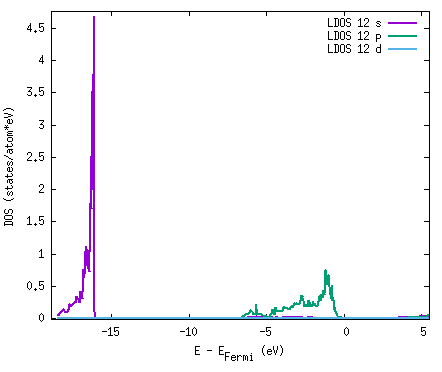
\includegraphics[width=\linewidth]{../fig/dosplot/ldos_O_II_primitive}\caption{This is a plot of local density of states at the O(II) site.}\label{fig:ldos_O_II}
\end{figure}

\begin{figure}[H]
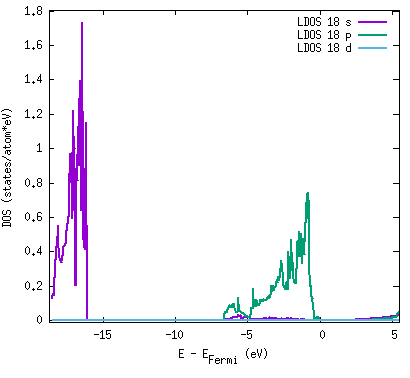
\includegraphics[width=\linewidth]{../fig/dosplot/ldos_O_III_primitive}\caption{This is a plot of local density of states at the O(III) site.}\label{fig:ldos_O_III}
\end{figure}

The structure has two different gallium sites as well, and their local density of states are shown in Figure \ref{fig:ldos_Ga_I} and \ref{fig:ldos_Ga_II}.

\begin{figure}[H]
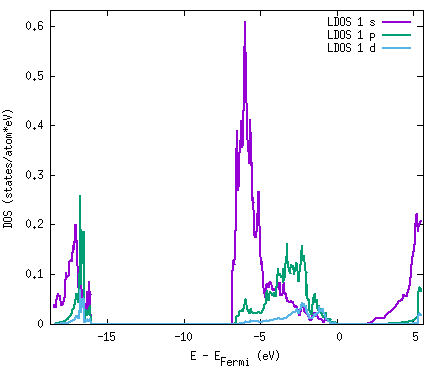
\includegraphics[width=\linewidth]{../fig/dosplot/ldos_Ga_I_primitive}\caption{This is a plot of local density of state at the Ga(I) site.}\label{fig:ldos_Ga_I}
\end{figure}

\begin{figure}[H]
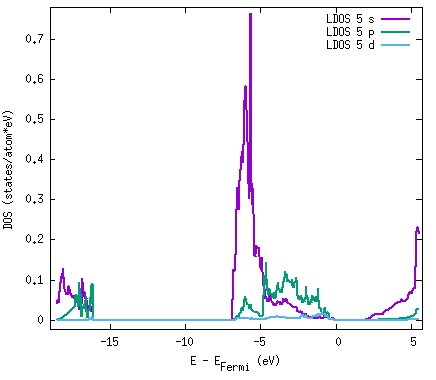
\includegraphics[width=\linewidth]{../fig/dosplot/ldos_Ga_II_primitive}\caption{This is a plot of local density of state at the Ga(II) site.}\label{fig:ldos_Ga_II}
\end{figure}

In the theory we can see that all the oxygen sites are 'bonded' to both gallium sites, but the number of each bonds differ (see \ref{fig:distances}). The p-orbitals with energy, $E-E_{Fermi}$, from -15 eV to 0 eV are in all the local density plots, both the gallium ones and the oxygen ones, indicating bonds between them all. There are also s-orbitals below -17 eV in all plots. There are many states there at the oxygen sites and fewer at the gallium sites. The gallium local DOS plots show some states in the d-orbitals, but oxygen do not, and that is of course what we expect.

\begin{figure}[H]
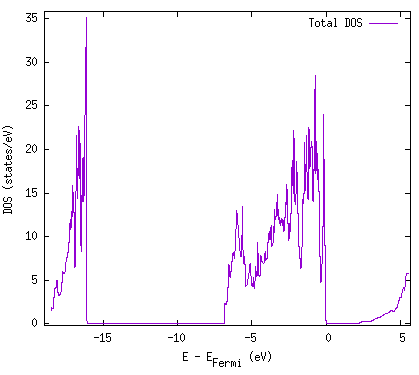
\includegraphics[width=\linewidth]{../fig/dosplot/total_DOS_primitive}\caption{This is a plot of density of state of the primitive unit cell.}\label{fig:total_dos_primitive}
\end{figure}

The total density of state of the primitive unit cell is plotted in Figure \ref{fig:total_dos_primitive}. The figures shows three bands in this energy interval, to bands below the Fermi level and the conduction band, of unoccupied states, as a semiconductor should have at temperature O K. The band gap is visual from 0 eV to around 2 eV, this is very small compared to experiments that gives the band gap at around 4.9 eV \cite{dft_ga2o3}. This is expected though because of the use of the simple GGA functional and no other compensation for the normal underestimation of band gap size.


\subsubsection{Band structure}

At last we plotted the band structure of $\beta$-Ga$_2$O$_3$. The band gap was found to be 1.8051 eV which is way too small. Figure \ref{fig:bandstructure_primitive} shows the band structure we plotted after our calculations. Figure \ref{fig:bandstructure_fasit} shows the band structure from an article where they used hybrid functionals and other tricks to get the correct band gap \cite{dft_ga2o3}. 

The band structure in Figure \ref{fig:bandstructure_primitive} shows that the lowest point in the conduction band is at the $\Gamma$-point (G), and this corresponds with the result in Figure \ref{fig:bandstructure_fasit}. The highest point in the valence band on our band structure is difficult to set, but in the other it is either at the M-point or the $\Gamma$-point.

There seems to be something wrong at the M-point in our calculations because it looks very different form the other one. The band gap of $\beta$-Ga$_2$O$_3$ is indirect, but the difference in the valence band between the $\Gamma$-point and the M-point is so small, that it is practically direct \cite{dft_ga2o3}.

\begin{figure}[H]\caption{This is a plot of the band structure of $\beta$-Ga$_2$O$_3$ form our density of states calculations.}\label{fig:bandstructure_primitive}
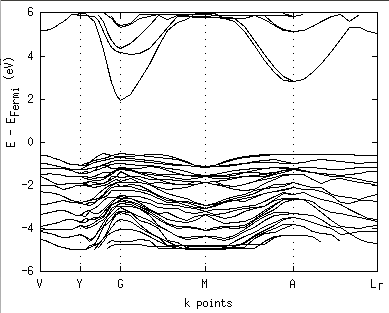
\includegraphics[width=\linewidth]{../fig/primitive/bandstructure}
\end{figure}

\begin{figure}[H]\caption{This is a plot of the band structure taken from an article that did DFT on $\beta$-Ga$_2$O$_3$ with hybrid density functionals \cite{dft_ga2o3}.}\label{fig:bandstructure_fasit}
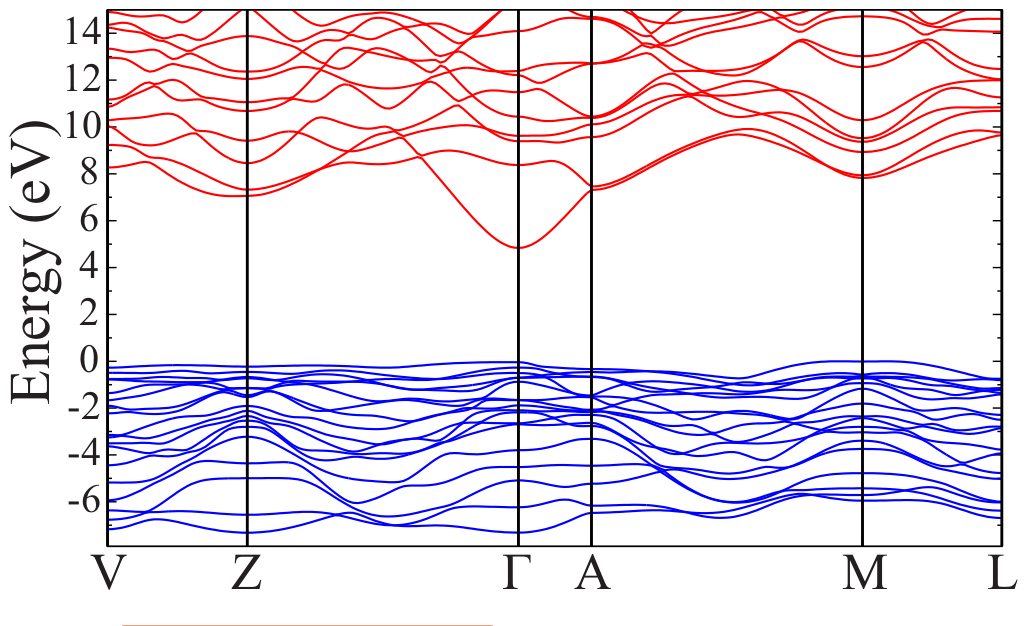
\includegraphics[width=\linewidth]{../fig/band_structure}
\end{figure}


\subsection{Super cell}

To be able to look at oxygen vacancies without getting extremely high concentrations of them, we increased the primitive cell to a super cell by adding two primitive cells in the y-direction (b-direction) and one in the z-direction (c-direction). 

\subsubsection{Relaxation and energy}

Our first relaxation of the unit cell was done with the initial convergence results of an energy cut-off at 600 eV and a k-point density at 5 Å$^{-1}$ giving a k-mesh of (3x4x3). The convergence for the maximum force was put to only -0.05 eV/Å (EDIFFG = -0.05) and we only relaxed the ions not the cell (ISIF = 2). The result of the relaxation is in Table \ref{tab:ionstep_convergence}.

\begin{table}[H]\caption{This table has the first and last relaxation step of supercell with the initial convergence result.}\label{tab:ionstep_convergence}
\begin{tabular}{rllll}
F$_{max}$ &\#$_{atom}$&	P&	Drift&	E$_{tot}$\\ \hline
0.443&	49&	134.07&	0.023&	-718.260\\
$\vdots$&$\vdots$&$\vdots$&$\vdots$&$\vdots$\\
0.009&	25&	109.22&	0.023&	-718.913\\
CPU &time: & 3546.421 s & & $\approx$ 59 min  \\
\end{tabular}
\end{table}

Because the pressure was so big, we wanted to relax the cell as well. We also wanted to decrease the convergence of the maximum force to 0.01 eV/Å (EDIFFG = -0.01) to match the convergence criteria of the force. Because the relaxation calculation was costly already, a decision to make the convergence criteria less strict was made. It was done like described earlier in the method part of this report. The total energy of the super cell after the initial relaxation is given in Table \ref{tab:energy_supercell_after_relax}.

Energy calculation after:
\begin{table}[H]\caption{The energy output after relaxation of supercell with first relaxation result.}\label{tab:energy_supercell_after_relax}
\begin{tabular}{llll}
F$_{max}$ & P&	Drift&	E$_{tot}$\\ \hline
\end{tabular}
\end{table}

\subsubsection{Changed convergence criteria}

The relaxation was then done with the changed convergence results with an energy cut-off at 500 eV and a k-point density at 3 Å$^{-1}$ giving a k-mesh of (2x3x2). The convergence for the maximum force was put to -0.01 eV/Å (EDIFFG = -0.01) and we relaxed both the ions and the cell (ISIF = 3). The result of the relaxation is in Table \ref{tab:ionstep_convergence_new} and the total energy of the super cell calculated from the relaxed structure is in Table \ref{tab:energy_supercell_after_relax_new}.

\begin{table}[H]\caption{This table has the first and last relaxation step of supercell with the changed convergence criteria.}\label{tab:ionstep_convergence_new}
\begin{tabular}{rllll}
F$_{max}$ &\#$_{atom}$&	P&	Drift&	E$_{tot}$\\ \hline
0.427&	49&	136.09&	0.023&	-717.821\\
$\vdots$&$\vdots$&$\vdots$&$\vdots$&$\vdots$\\
0.006&	49&	0.03&	0.024&	-720.914\\
\end{tabular}
\end{table}

\begin{table}[H]\caption{The energy output after last relaxation of supercell.}\label{tab:energy_supercell_after_relax_new}
\begin{tabular}{llll}
F$_{max}$ & P&	Drift&	E$_{tot}$\\ \hline
0.045&	0.023&	2.63	&-721.081\\
\end{tabular}
\end{table}

The total energy per atom with the super cell was $\frac{E_{tot}}{\# \text{ of atoms}} = \frac{-721.081 \text{ eV}}{120} \simeq -6.009 \text{ eV}$ after the relaxation. The energy per atom is the same as for the primitive unit cell, within the chosen accuracy. 

\subsection{O$_2$ in vacuum}

To calculate the formation energy we need the energy of oxygen in vacuum. This energy was calculated with the same cut-off energy as before and the k-point density 1 Å$^{-1}$ which gives the k-mesh (1x1x1) because it is only one molecule with vacuum in all directions. O$_2$ has a paramagnetic ground state, so we had to turn on the spin -polarization (ISPIN = 2). We relaxed the structure (Table \ref{tab:oxygen_relax} and then calculated the total energy (see Table \ref{tab:oxygen_vacuum}).

\begin{table}[H]\caption{This table has relaxation steps of =$_2$ in vacuum.}\label{tab:oxygen_relax}
\begin{tabular}{rllll}
F$_{max}$ &\#$_{atom}$&	P&	Drift&	E$_{tot}$\\ \hline
0.087&	1&	-0.22&	0.000&	-9.883\\
0.406&	1&	0.09&	0.000&	-9.882\\
0.000&	1&	-0.16&	0.000&	-9.883\\
\end{tabular}
\end{table}

\begin{table}[H]\caption{The energy output of oxygen in vacuum.}\label{tab:oxygen_vacuum}
\begin{tabular}{llll}
F$_{max}$ &	P&	Drift&	E$_{tot}$ \\ \hline

\end{tabular}
\end{table}

From this energy we can calculate the chemical potential, at our conditions, using Equation \ref{eq:mu_O_simple}:

$$ \mu_O = \frac{1}{2}E_{tot}^{O_2} = \frac{1}{2}\cdot(-9.883) = -4.942 $$

\subsection{The different oxygen vacancies}

Furthermore, we removed an oxygen atom from the three different sites, relaxed the structures and calculated the total energy of the structures. The same parameters were used in these as the calculations of the super cell without vacancies.

\subsubsection{Relaxation}

Table \ref{tab:ionstep_O_I} shows the first and last ionstep of the relaxation of the super cell with a O(I) vacancy. Table \ref{tab:ionstep_O_II} and Table \ref{tab:ionstep_O_III} shows the same for the O(II) vacancy and the O(III) vacancy respectively.

\begin{table}[H]\caption{The ionstep - relaxation of super cell with O(I) vacancy.}\label{tab:ionstep_O_I}
\begin{tabular}{rllll}
F$_{max}$ &\#$_{atom}$&	P&	Drift&	E$_{tot}$\\ \hline
2.666&	19&	133.08&	0.142&	-708.492\\
$\vdots$&$\vdots$&$\vdots$&$\vdots$&$\vdots$\\
0.032&	63&	-0.03&	0.465&	-712.142\\
\end{tabular}
\end{table}

\begin{table}[H]\caption{The ionstep - relaxation of super cell with O(II) vacancy.}\label{tab:ionstep_O_II}
\begin{tabular}{rllll}
F$_{max}$ &\#$_{atom}$&	P&	Drift&	E$_{tot}$\\ \hline
2.391&	20&	135.21&	0.010&	-708.256	\\
$\vdots$&$\vdots$&$\vdots$&$\vdots$&$\vdots$\\
0.013&	60&	-0.01&	0.143&	-711.709\\
\end{tabular}
\end{table}

\begin{table}[H]\caption{The ionstep - relaxation of super cell with O(III) vacancy.}\label{tab:ionstep_O_III}
\begin{tabular}{rllll}
F$_{max}$ &\#$_{atom}$&	P&	Drift&	E$_{tot}$\\ \hline
1.873&	1&	135.42&	0.141&	-707.966	\\
$\vdots$&$\vdots$&$\vdots$&$\vdots$&$\vdots$\\
0.017&	73&	-0.00&	0.145&	-711.463	\\
\end{tabular}
\end{table}

\subsubsection{Total Energy}

The total energy and other output of the relaxed structures are in Table \ref{tab:energy_supercell_vacancies}.

\begin{table}[H]\caption{The energy output after relaxation of supercell with oxygen vacancies.}\label{tab:energy_supercell_vacancies}
\begin{tabular}{l|llll}
Vacancy& F$_{max}$ &	P&	Drift&	E$_{tot}$ \\ \hline
O(I)&    0.107&	    0.146&	2.29	&    -712.283\\
O(II)&    0.067&	    0.198&	2.39	&    -711.860\\
O(III)&    0.087&    0.221&	2.13	&    -711.603\\
\end{tabular}
\end{table}

\subsubsection{Formation Energy}

We used Equation \ref{eq:formation_energy} to calculate the formation energy of the three different situations and find which of the vacancies that had the smallest formation energy. 

\begin{table}[H]\caption{This is the calculated formation energies for the diffrent oxygen vacancies at oxygen rich conditions. $E_f$ is the formation energy, $E_{vac}$ is the total bulk energy with the spesicied vacancy, $E_b$ is the total bulk energy without a vacancy and $\mu_O$ is the chemical potential of oxygen. }\label{tab:energy_formation}
\begin{tabular}{l|rl}
\footnotesize Vacancy&$(E_{vac} + \mu_O)- E_b = $ &$E_f$ \\ \hline
\small O(I)&$(-712.282 -4.942)-721.081 =$ &3.857\\
\small O(II)&$(-711.860 -4.942)-721.081 =$ &4.279\\
\small O(III)&$(-711.603 -4.942)-721.081 =$ &4.536\\
\end{tabular}
\end{table}

From Table \ref{tab:energy_formation} we can read that the O(I) vacancy has the lowest formation energy at the conditions we are checking at.

\subsection{Why the O(I) vacancy?}

We will use isosurfaces and local DOS to evaluate why the O(I) vacancy is the one with smallest formation energy.

\subsubsection{Total density of states}

First we can see that a defect level has showed up in the band gap, probably from the oxygen vacancy. This is shown when comparing Figure \ref{fig:total_dos_vac} which is the total DOS of the supercell without vacancies and \ref{fig:total_dos_supercell} which is DOS of the supercell with the O(I) vacancy.

\begin{figure}[H]
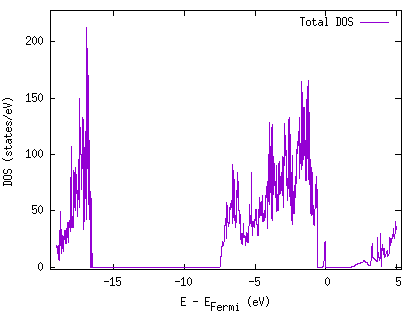
\includegraphics[width=\linewidth]{../fig/dosplot/total_dos_O_I_vacancy}\caption{This is a plot of the density of state of the super cell with a O(I) vacancy.}\label{fig:total_dos_vac}
\end{figure}

\begin{figure}[H]
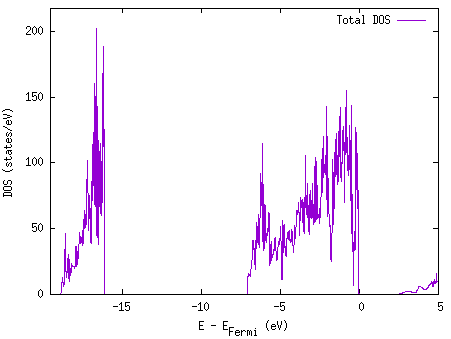
\includegraphics[width=\linewidth]{../fig/dosplot/total_dos_supercell}\caption{This is a plot of density of state of the general supercell.}\label{fig:total_dos_supercell}
\end{figure}

\subsubsection{Isosurfaces}

Figure \ref{fig:isosurface_O_I} shows the structure around the O(I) vacancy with different electron density isosurface levels. When the isosurface level is set to 0.04, an electron density is visible between the two Ga(I) atoms the O(I) atom should have been bonded to and and when the isosurface level is 0.03, the isosurface shows a bond between them (Figure \ref{fig:bond_O_I}).

\begin{figure}[H]
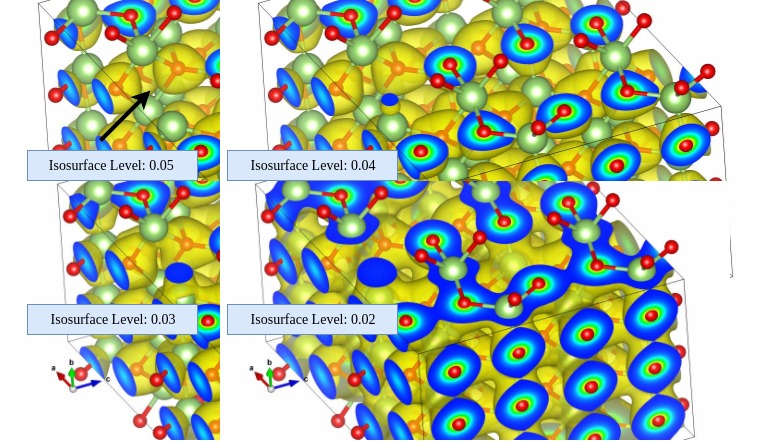
\includegraphics[width=0.9\linewidth]{../fig/isosurfaces/O_I/isosurface}\caption{This figure shows the O(I) vacancy with different electron density isosurfaces.The black arrow points to the O(I) vacancy. When the isosurface level is lowered, a bond appears between the two Ga(I) atoms the O(I) should have been bonded to (Figure \ref{fig:bond_O_I}).}\label{fig:isosurface_O_I}
\end{figure}

\begin{figure}[H]
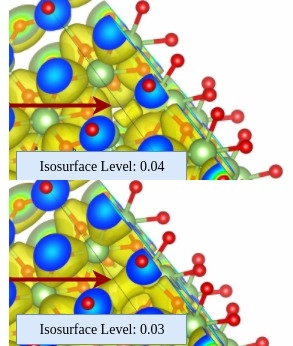
\includegraphics[width=0.7\linewidth]{../fig/isosurfaces/O_I/bond}\caption{This figure shows the oxygen vacancy with different isosurfaces.In this figure the bond between the two Ga(I) atoms shows clearly. The isosurface goes from one atom to the other at the isosurface level 0.03.}\label{fig:bond_O_I}
\end{figure}

Figure \ref{fig:isosurface_O_II} shows the O(II) vacancy with different isosurfaces, when the isosurface level is lowered, the electron density around the Ga(I)-atom shows. The 'blob' shows the dangling bonds at the Ga(I) atom, but there is no 'blob' at the Ga(II) atoms. With the O(II) vacancy the isosurface level needs to be 0.02 for there to be a connection with the other Ga(II) atoms.

\begin{figure}[H]
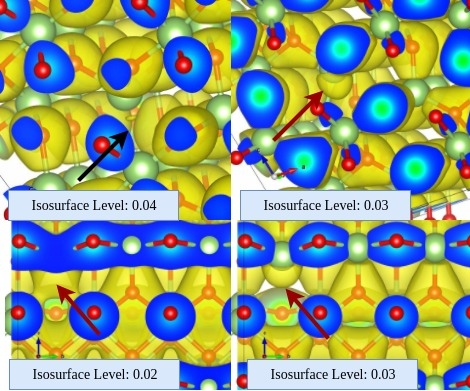
\includegraphics[width=\linewidth]{../fig/isosurfaces/O_II/isosurface}\caption{This figure shows the O(II) vacancy with different electron density isosurfaces.The figure shows the oxygen vacancy from different angles. The black arrow points to the vacancy and the red arrows points to the isosurface indicating dangling bonds at the Ga(I) atom.}\label{fig:isosurface_O_II}
\end{figure}

Figure \ref{fig:isosurface_O_III} shows the same for the O(III) vacancy. As in the case for the O(II) vacancy, the isosurface level needs to be 0.02 before there is a connection, and before that there is the same 'blob' at the one Ga(I) atom, indication dangling bonds.

\begin{figure}[H]
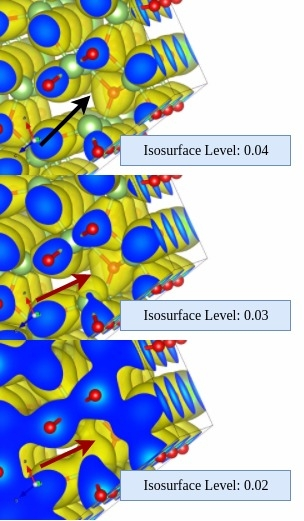
\includegraphics[width=0.7\linewidth]{../fig/isosurfaces/O_III/isosurface}\caption{This figure shows the oxygen vacancy with different electron density isosurfaces.The black arrow points to the oxygen vacancy and the red arrows points to the dangling bond at the Ga(I) atom.}\label{fig:isosurface_O_III}
\end{figure}

The difference between the O(I) vacancy with two Ga(I) atoms, that seems to form a covalent bond in the absence of an oxygen, and the other two vacancies, that only have one Ga(I) atom, might be a reason why the O(I) vacancy has the lowest formation energy.

The reason for the bond between two the Ga(I) atoms may come from the shorter length of the O-Ga(I) bond compared to the O-Ga(II) bond (see Figure \ref{fig:distances}). The 'bulb' from the isosurface always occur at the Ga(I) atom, and nothing at the Ga(II) atoms. Maybe the Ga(I) atom has dangling bonds, and the Ga(II) relocate the electrons elsewhere, making the O(I) more stable because the dangling bonds are in a bond instead. 

\subsubsection{Local DOS Ga(II)}

lDOS - bredden sier om båndene er bånd - ikke så lokaliserte. Bånd til venstre er mer stabile - lenger borte fra fermi nivået.

\begin{figure}[H]
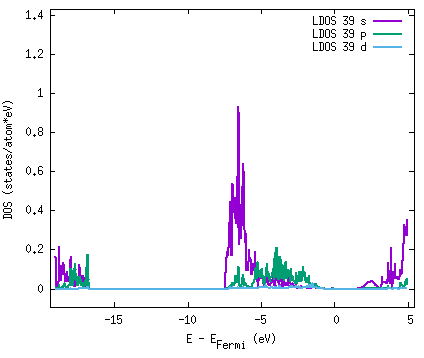
\includegraphics[width=\linewidth]{../fig/dosplot/ldos_Ga_II_OI_vac_nabo}\caption{This is a plot of local density of state at the Ga(II) site next to the O(I) vacancy in the super cell.}\label{fig:ldos_Ga_II_nabo}
\end{figure}

\begin{figure}[H]
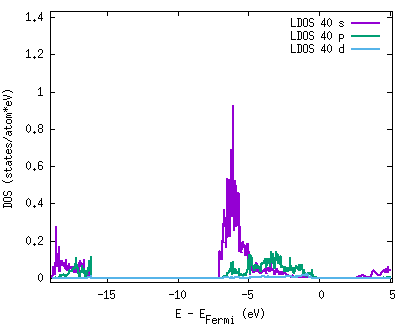
\includegraphics[width=\linewidth]{../fig/dosplot/ldos_Ga_II_supercell}\caption{This is a plot of local density of state at the Ga(II) site in the general supercell.}\label{fig:ldos_Ga_II_supercell}
\end{figure}

\subsubsection{Local DOS Ga(I)$_1$}

\begin{figure}[H]
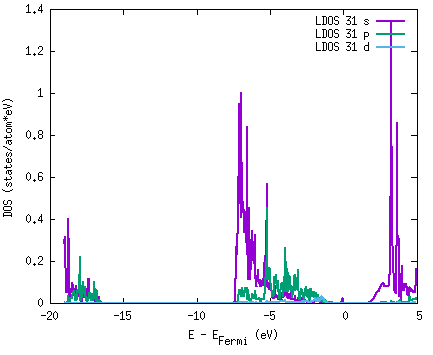
\includegraphics[width=\linewidth]{../fig/dosplot/ldos_Ga_I_OI_vac_nabo}\caption{This is a plot of local density of state at the Ga(I) site next to the O(I) vacancy in the super cell.}\label{fig:ldos_Ga_I_nabo}
\end{figure}

\begin{figure}[H]
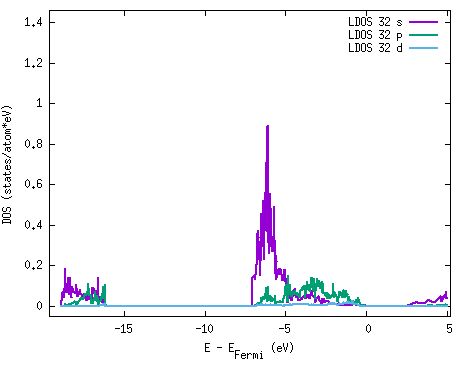
\includegraphics[width=\linewidth]{../fig/dosplot/ldos_Ga_I_supercell}\caption{This is a plot of local density of state at the Ga(I) site in the general supercell.}\label{fig:ldos_Ga_I_supercell}
\end{figure}

\subsubsection{Bond between Ga(I)$_1$ and Ga(I)$_2$?}

\begin{figure}[H]
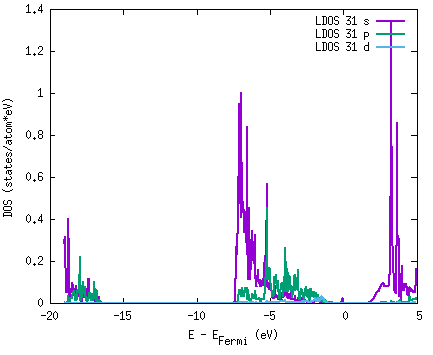
\includegraphics[width=\linewidth]{../fig/dosplot/ldos_Ga_I_OI_vac_nabo}\caption{This is a plot of local density of state at the Ga(I) site next to the O(I) vacancy in the super cell.}\label{fig:ldos_Ga_I_nabo}
\end{figure}

\begin{figure}[H]
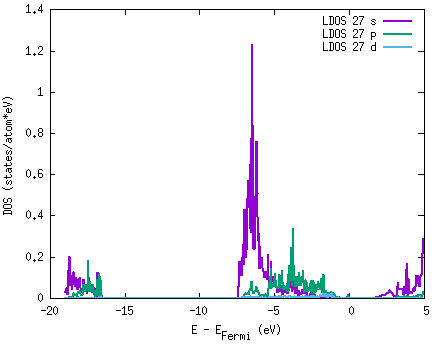
\includegraphics[width=\linewidth]{../fig/dosplot/ldos_Ga_I_OI_vac_nabo2}\caption{This is a plot of local density of state at the other Ga(I) site next to the O(I) vacancy in the super cell.}\label{fig:ldos_Ga_I_nabo}
\end{figure}

